\documentclass[a4paper,11pt]{article}

\usepackage[slovene]{babel}
\usepackage[utf8]{inputenc}

\usepackage{listings}
\usepackage{babelbib}
\usepackage{url}

\usepackage{graphicx}
\graphicspath{ {images/} }
\usepackage[usenames, dvipsnames]{color}

\usepackage{underscore}
\renewcommand{\lstlistingname}{Primer}% Listing -> Primer

\lstset{
numbers=left, 
numberstyle=\small, 
numbersep=8pt, 
frame = single, 
language=Python, 
framexleftmargin=15pt}

\setlength{\parindent}{0pt}
%BORDERS
\usepackage{geometry}
 \geometry{
 a4paper,
 total={170mm,257mm},
 left=30mm,
 right=25mm,
 top=30mm,
 bottom=30mm
 }

\begin{document}
\begin{titlepage}


% ZAČETNA STRAN
\newcommand{\HRule}{\rule{\linewidth}{0.5mm}} % Defines a new command for the horizontal lines, change thickness here

\center % Center everything on the page
 
%----------------------------------------------------------------------------------------
%	HEADING SECTIONS
%----------------------------------------------------------------------------------------

\textsc{ UNIVERZA V MARIBORU\\ FAKULTETA ZA ELEKTROTEHNIKO,\\RAČUNALNIŠTVO IN INFORMATIKO}\\[5cm] % Name of your university/college

%----------------------------------------------------------------------------------------
%	TITLE SECTION
%----------------------------------------------------------------------------------------
{ \huge \bfseries \textbf{KONEC SPRINTA 4}}\\[0.4cm] % Title of your document
\textsc{\large Povezljivi sistemi in inteligentne storitve}\\[5cm] % Minor heading such as course title

%----------------------------------------------------------------------------------------
%	AUTHORS SECTION
%----------------------------------------------------------------------------------------
{\large Gašper Gračner}\\[0.4cm]
{\large Martin Oprešnik}\\[0.4cm]
{\large Luka Koštomaj}\\[0.4cm] 

%----------------------------------------------------------------------------------------
%	DATE SECTION
%----------------------------------------------------------------------------------------
\vfill % Fill the rest of the page with whitespace
{\large Maribor, Maj 2016}\\[3cm] % Date, change the \today to a set date if you want to be precise
\end{titlepage}
\newpage

%----------------------------------------------------------------------------------------
%	CONTENT SECTION
%----------------------------------------------------------------------------------------

\section{Predvidene naloge}
V četrtem sprintu smo si vsi zadali analizo oz. testiranje izbranih metod strojnega učenja.
	\begin{enumerate}
		\item{Gašper Gračner - Uporaba različnih implementacij SVM - \textcolor{Orange}{Changed}, }
		\item{Luka Koštomaj - dodajanje šuma in podpora predlaganju treningov - \textcolor{OliveGreen}{DONE}, }
		\item{Martin Oprešnik - implementacija ansambelske metode - \textcolor{Orange}{Changed}}
	\end{enumerate}
Prvič, se je zgodilo, da nismo sledili načtru izdelanem na začetku, saj je prišlo do določenih zapletov pri implementaciji predlaganja treningov, zato je bilo potrebno delo prerazporediti.
	

\newpage
\section{Gašper Gračner - implemetacija predlaganja treningov}
Prvotna ideja predlaganja, ki je predvidila naključno genereiranje treningov, je bila opuščena. Izdelali smo sistem predlaganja, ki lahko kot vhodne parametre sprejme omejitve za posameznika in glede na te omejitve poskuša sestaviti primeren trening iz že obstoječih podatkov.\
Parametri, ki jih sprejeme:
\begin{itemize}
	\item{min intensity,}
	\item{max intensity,}
	\item{min duration,}
	\item{max duration,}
	\item{min heath rate,}
	\item{max heath rate,}
	\item{training days}
\end{itemize}

\section{Luka Koštomaj - dodajanje šuma in podpora predlaganju treningov}
V zadnjem sprintu sem dodal še predlaganje nevronskih mrež. To je predvsem dopolnitev tega kar je naredil Gašper. Dodal sem tudi nekaj šuma ali nepravilnih podatkov v našo podatkovno bazo. Klasifikacija podatkov je trenutno binarna. Za dodajanje šuma sem samo klasificiral narobe.


\section{Martin Oprešnik - implementacija ansambelske metode}
Ker smo v zadnjem sprintu v podatke vnesli šum, so klasifikatorji izgubili na natančnosti, zato smo želeli poskusiti še z ansambelsko metodo. Preizkusil sem metodo AdaBoost, a ni prinesla izboljšav v primerjavi z odločitvenim drevesom. Poleg tega sem dodal podporo za priporočanje na podlagi odločitvenega drevesa in ansambelske metode, kar je prilagoditev kode, ki jo je napisal Gašper.

\newpage
\section{Zaključek}
Po četrtem sprintu lahko trdimo, da smo uspešno končeli projekt, dosegli smo vse "Milestones", na glavnem branchu smo trije contributorji dosegli 47 commitov.


\begin{figure}[h]
\caption{Zaslonska slika končanih milestones-ov}
\centering
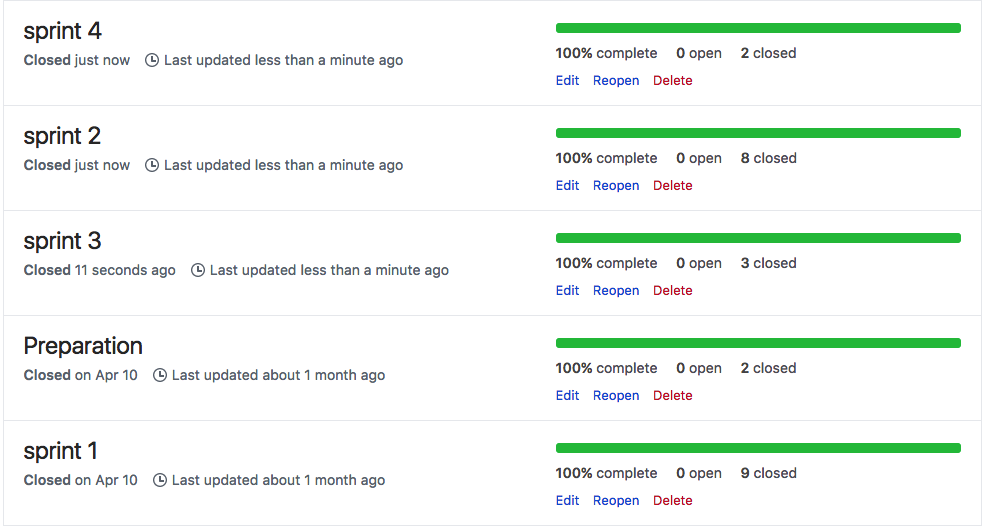
\includegraphics[width=1\textwidth]{closedsprints}
\end{figure}





\end{document}